\section{设计规划}

\subsection{设计要求}

\subsubsection{设计内容}

设计一个打地鼠游戏机. 本设计在原题要求上进行了一定的扩展, 使得游戏机具有更好的可玩性. 下面是本设计的主要功能:

\begin{itemize}
    \item 用 HDMI 显示地鼠, 当前的难度以及得分情况.
    \item 有一个 Start 按钮用于控制游戏开始, 一个 Reset 按钮用于重置游戏.
    \item 游戏开始后, 会在屏幕上显示地鼠, 地鼠间隔一定的随机时间 $T_1$ 刷新位置并显示, 并持续 $T_2$ (随难度变化)时间. 
    \item 游戏分为 3 轮, 每轮游戏结束后若超过规定分数, 则进入下一轮. 在每轮游戏中, 打到地鼠得到的分数随难度增加而增加.
    \item 游戏结束后, 显示总分. 
\end{itemize}

\subsection{设计思路}

\subsubsection{硬件设计}

我采用 SpinalHDL 完成硬件设计部分. SpinalHDL 是一种基于 Scala 的硬件描述语言, 
可以生成 VHDL 或 Verilog 文件, 以此与现有的 EDA 工具兼容. 借由 Scala 提供的现代高级
编程语言的特性, SpinalHDL 可以大大提高硬件设计的效率. 它\textbf{不是}一种高层次综合语言, 
也非基于事件驱动的范式. 它依然是一种基于寄存器传输级 (RTL) 的描述范式. 

我采用 SpianlHDL 的原因在于其适用于快速开发迭代流程, 并提供良好的封装和代码可读性. 可以将
各个组件低耦合地设计, 并在最后组合起来. 它还提供了强大的参数化设计能力, 而这一点是在 Verilog
中很难做到的. 

\lstinputlisting[language=scala, caption={SpinalHDL 实现的加法器}, label={code:spinalexample}]{res/code/exampleOfSpinal.scala}

如代码\ref{code:spinalexample} 所示是一个简单的 SpinalHDL 示例, 其实现了一个位宽参数化的加法器. 



\subsubsection{软件仿真}

我使用了 Verilator 作为基本仿真工具并结合 Qt 作为图形化界面. 
Verilator 是一个开源的 Verilog仿真器, 它可以将 Verilog 代码编译成 C++ 代码, 并提供了一套 C++ API 用于仿真. 其优点在于
仿真速度快, 且可以方便地与 C++ 代码进行交互. Qt 是一个跨平台的 GUI 库, 可以方便地实现图形化界面. 通过
读取 Verilator 生成的仿真结果, 我可以在 C++ 中读取每一个周期的 RGB, VSYNC, HSYNC 信号, 并将其进行拼接, 
最终在软件端模拟一个显示器进行显示. 仿真器如图 \ref{fig:emulator} 所示. 

\begin{figure}
    \centering
    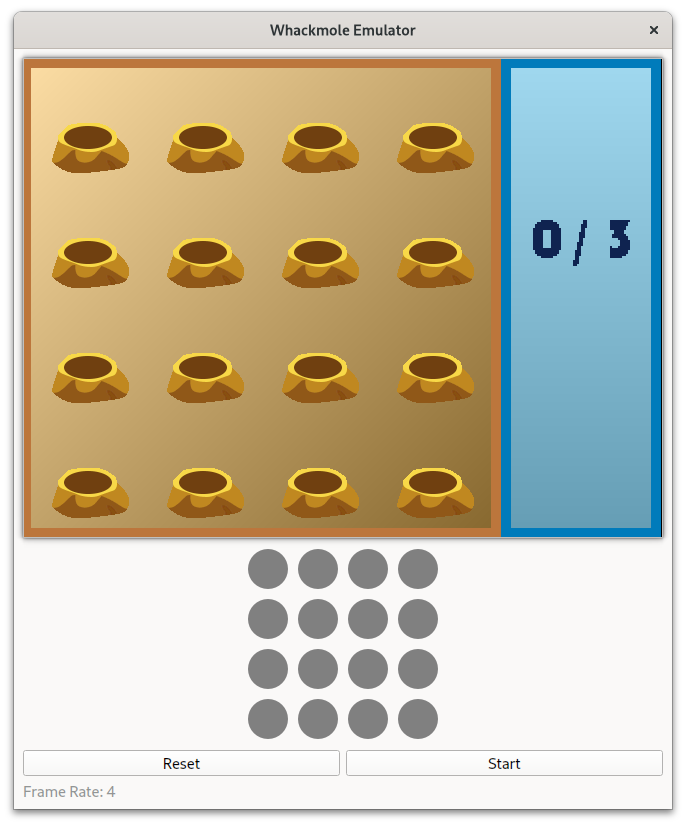
\includegraphics[width=0.5\textwidth]{res/img/emulator.png}
    \caption{以 Verilator 为基础的软件仿真器}
    \label{fig:emulator}
\end{figure}

显然, 软件端的模拟不可能达到硬件端的速度. 我采用的是640x480的分辨率, 以 60Hz 的刷新率进行显示的时序. 然而, 
软件端只能做到以 10Hz 的刷新率进行显示. 为了保证软件运行的稳定性(过高的刷新率容易导致处理跟不上, 从而使得
跨线程信号堆积), 我把软件的刷新率固定在了 5Hz. 那么, 我们怎么保证在时钟频率不同的硬件端和软件端游戏体验一致呢? 

好在, SpinalHDL 为我们提供了一套封装, 让我可以使用"秒"和"频率"作为参数进行设计. 如代码 \ref{code:spinaltime} 所示. 
这段代码是我实际使用的代码. 

\begin{lstlisting}[caption={SpinalHDL 中的时间参数}, label={code:spinaltime}, language=scala]
val frequency: HertzNumber = 2 MHz,
val roundGapTime: TimeNumber = 3 sec,
\end{lstlisting}

我向软件端传输的是 VGA 信号, 则刷新一帧需要 $525 \times 800 = 420000$ 个周期. 在 2 MHz 的
像素时钟下, 一帧需要 $420000 / 2000000 = 0.21$ 秒. 这样就能适应软件端 5 Hz 的刷新率.

如果要在硬件端实现, 我只需要将 2 MHz 改变为标准时钟频率 25.175 MHz 即可. 所有的时间参数, 例如
各轮之间的时长都不需要做任何额外的代码修改就能保持一致. 

\subsection{设计流程图及 EDA 使用说明}

设计流程图如图 \ref{fig:flowpath} 所示.

\begin{figure}
    \centering
    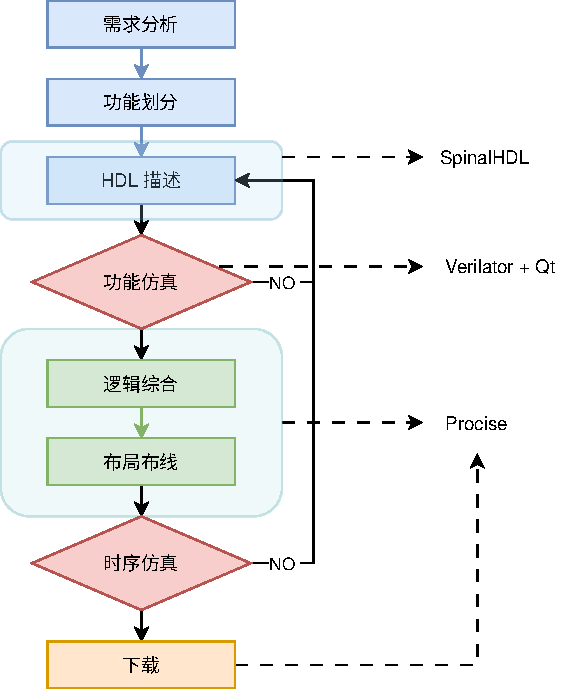
\includegraphics[width=0.5\textwidth]{res/img/flowpath.pdf}
    \caption{Top--Down 设计流程图}
    \label{fig:flowpath}
\end{figure}

本次设计的 FPGA 上板验证采用复微开发的 FPGA 开发板. 我也使用了 Procise 作为 EDA 工具进行综合和布局布线.

课程提供的工程示例对我帮助很大. 我在其基础上学习使用了 Procise 工具的使用方法, 掌握了该 EDA 工具的使用流程. 
